\documentclass[border=4pt]{standalone}
\usepackage{fontspec}
\usepackage{amsmath}
\usepackage{unicode-math}
\setmainfont{Latin Modern Roman}
\setmathfont{Latin Modern Math}
\usepackage{pgfplots}
\usepackage{pgfplotstable}
\pgfplotsset{compat=1.18}
\usepackage{tkz-euclide}
\usetikzlibrary{arrows.meta,calc,angles,quotes,patterns,3d,backgrounds}
\definecolor{ink}{HTML}{123428}
\definecolor{asy}{HTML}{475569}
\definecolor{mint}{HTML}{86e0bd}
\tikzset{asym/.style={asy, line width=0.9pt, dash pattern=on 5pt off 3.5pt},
         guide/.style={gray!70, line width=0.6pt, densely dotted},
         dot/.style={circle, inner sep=0pt, minimum size=5pt, draw=white, line width=0.5pt},
         odot/.style={circle, inner sep=0pt, minimum size=5.5pt, fill=white, line width=1pt},
         lab/.style={font=\footnotesize, inner sep=1.5pt, text=ink}}
\begin{document}
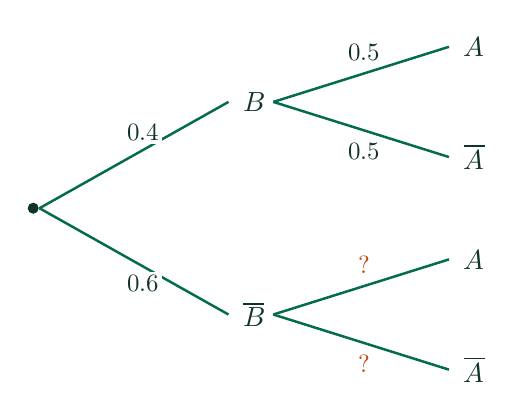
\begin{tikzpicture}[x=1cm,y=1cm]
\draw[color={rgb,255:red,4;green,107;blue,77}, line width=0.9pt] (0.08,0.00) -- (2.48,1.35);
\node[font=\small, text=ink, fill=white, inner sep=1pt] at (1.40,0.96) {$0.4$};
\draw[color={rgb,255:red,4;green,107;blue,77}, line width=0.9pt] (0.08,0.00) -- (2.48,-1.35);
\node[font=\small, text=ink, fill=white, inner sep=1pt] at (1.40,-0.96) {$0.6$};
\draw[color={rgb,255:red,4;green,107;blue,77}, line width=0.9pt] (3.05,1.35) -- (5.28,2.05);
\node[font=\small, text=ink, fill=white, inner sep=1pt] at (4.20,1.98) {$0.5$};
\draw[color={rgb,255:red,4;green,107;blue,77}, line width=0.9pt] (3.05,1.35) -- (5.28,0.65);
\node[font=\small, text=ink, fill=white, inner sep=1pt] at (4.20,0.72) {$0.5$};
\draw[color={rgb,255:red,4;green,107;blue,77}, line width=0.9pt] (3.05,-1.35) -- (5.28,-0.65);
\node[font=\small, text={rgb,255:red,194;green,65;blue,12}, fill=white, inner sep=1pt] at (4.20,-0.72) {$?$};
\draw[color={rgb,255:red,4;green,107;blue,77}, line width=0.9pt] (3.05,-1.35) -- (5.28,-2.05);
\node[font=\small, text={rgb,255:red,194;green,65;blue,12}, fill=white, inner sep=1pt] at (4.20,-1.98) {$?$};
\fill[ink] (0,0) circle (2pt);
\node[text=ink] at (2.80,1.35) {$B$};
\node[text=ink] at (2.80,-1.35) {$\overline{B}$};
\node[text=ink] at (5.60,2.05) {$A$};
\node[text=ink] at (5.60,0.65) {$\overline{A}$};
\node[text=ink] at (5.60,-0.65) {$A$};
\node[text=ink] at (5.60,-2.05) {$\overline{A}$};
\end{tikzpicture}
\end{document}
